\documentclass[a4paper, 12pt]{article}
% \documentclass[draft, 12pt]{article}
\usepackage[utf8]{inputenc}
\usepackage[brazilian]{babel}
\usepackage{graphicx}
\usepackage{amssymb, mathrsfs, amsfonts, amsmath, esint, relsize, bm}
\usepackage{hyperref}
\usepackage{caption}
\usepackage{indentfirst} 
\usepackage{xcolor}
\usepackage{csquotes} % When using babel or polyglossia with biblatex, loading csquotes is recommended to ensure that quoted texts are typeset according to the rules of your main language.
% References
\usepackage[style=ieee]{biblatex}
\addbibresource{refs.bib}

% \usepackage{hhline}
% \usepackage{color}
% \usepackage{soul}
% \usepackage[table,xcdraw]{xcolor}
% \usepackage{enumerate}

%% My commands
% \newcommand{\myref}[1]{{\color{blue} \ref{#1}}} % Display a blue color for linking figures, tables, equations, etc..
% \newcommand{\mywidth}{.6} % Standard for figures
% \hypersetup{linkcolor=blue, filecolor=magenta, urlcolor=cyan}

% Change background color
% \usepackage{pagecolor,lipsum}% http://ctan.org/pkg/{pagecolor,lipsum}

% \definecolor{maroon}{cmyk}{0,0.87,0.68,0.32}

\begin{document}
% \pagecolor{yellow!50!orange} % ``marcador'' de página feita (movimentas ou comentá-lo de acordo com o avanço do trabalho)

%--------------------------------------------------------------------------
% Capa do relatório
\begin{titlepage}
    \begin{center}
        
\includegraphics[width=2cm]{adj/brasao.png}\\
        {\large {Universidade Federal do Ceará}}\\
        {\large {Centro de Tecnologia}}\\
        {\large {Departamento de Engenharia de Teleinformática}}\\
        {\large {Sistemas de Comunicações Digitais - TI0069}}
    \end{center}

    \vspace{100pt}
    
    \begin{center}
        {\large \textbf {Trabalho 01: Modulação Digital}}
    \end{center}
    
    \vspace{100pt}
    
    \begin{table}[h]
    \begin{tabular}{ll}
        \textbf{Aluno:}         &       \\
        Lucas de Souza Abdalah  & 385472
    \end{tabular}
    \end{table}
    
    \begin{table}[h]
    \begin{tabular}{l}
        \textbf{Professor:} André Almeida   \\
        \textbf{Data de Entrega do Relatório:} 28/03/2021
    \end{tabular}
    \end{table}
    
    \vspace{\fill}
    
    \begin{center}
        Fortaleza\\
        2021
    \end{center}
    
    \end{titlepage}
    
    %--------------------------------------------------------------------------
    % Sumario do relatorio
    
    \tableofcontents
    \thispagestyle{empty}
    \clearpage

% Exemplo de citação usando \cite{}
%--------------------------------------------------------------------------
% Exemplos
\section*{Exemplos}

% Place holder de texto
% \lipsum[1]

Para referenciar imagens~\ref{fig:brasao_UFC}, tabelas~\ref{tab:frequencia_tensao} e equações~\ref{eq:frequencia_ganho}.

\begin{figure}[!ht]
    \centering
    
\includegraphics[width=0.15\textwidth]{adj/brasao.png}
    \caption{Exemplo de como adicionar uma imagem.}
    \label{fig:brasao_UFC}
\end{figure}

\begin{table}[!ht]
    \centering
    \begin{tabular}{|c|c|}
    \hline
    Frequência (Hz) & Tensão Máxima (V) \\ \hline
    0,558            & 12,11            \\ \hline
    2,132            & 11,15            \\ \hline
    4,822            & 8,62             \\ \hline
    \end{tabular}
    \caption{Frequência da onda de entrada e a tensão máxima da saída do circuito integrador.}
    \label{tab:frequencia_tensao}
\end{table}

\begin{equation}
    f_{gu} = A_{VD}\times f_{c}
    \label{eq:frequencia_ganho}
\end{equation}

% Exemplo de citação usando \cite{}
E quando tirar informação de alguma fonte, deve adicionar no formato de bibtex no arquivo refs.bib e por fim citá-los assim:~\cite{Fonseca}, de modo que a seção de referência é criada e indexada diretamente com estes chamados da função.

\clearpage

\section{Introdução}
% \clearpage

\section{Simulações}
\subsection{Problema 1 - \texorpdfstring{$M$}{M}-QAM}

Considere a modulação $M$-QAM, em que o sinal em banda base é dado por:
$$s_m(t) = ( A_m^{(\text{real})} + j A_m^{(\text{imag})}) g(t) ,$$
em que $g(t)$ é um pulso transmitido, $A_m^{(\text{real})}$ e $A_m^{(\text{imag})}$ são amplitudes da parte real e imaginária da forma de onda transmitida, respectivamente.

% Considere $\int_{-\inf}^{\inf} |g(t)|^2 \,dt = \mathcal{E}_{g} = 1$, isto é, o pulto $g(t)$ possui energia unitária. Suponha a transmissão de uma sequência de símbolo $\{s_{m}\}$ de tamanho $L = 26400 \text{bits}$
% \begin{enumerate}
%     \item A energia média $\mathcal{E}_{m}$ de cada constelação;
%     \item A distância mínima $d_{min}$ entre dois símbolos;
%     \item O modulador (mapeamento bit-símbolo) usando a codificação de Gray;
%     \item O demodulador (mapeamento símbolo-bit).
% \end{enumerate}

% -------------------------------------------------------------------

\subsubsection{Energia da Constelação} 

O desenvolvimento é citado em~\cite{Proakis, Cecilio}.

$$ \mathcal{E}_{media} = \frac{M-1}{3} \mathcal{E}_g$$

$$ \mathcal{E}_{media(bit)} = \frac{M-1}{3\log_2 M} \mathcal{E}_g $$
% -------------------------------------------------------------------
\subsubsection{Distância Mínima entre Símbolos}

Como calcular os coeficiente para constelação $M$-QAM retangular, onde $\sqrt{M}$ assume valores inteiros. Os coeficientes em quadratura $a_i$ e $b_i$ são obtidos através da equação: $\{ (2i -\sqrt{M} - 1)d \}_{i=1}^{\sqrt{M}} $ 

A distância eucliadiana entre os sinais na modulação QAM é
$$ d_{mn} = \sqrt{|| s_m - s_n||^2}$$ 
$$ = \sqrt{\frac{\mathcal{E}_g}{2}[(A_{mi} - A_{ni})^2 + (A_{mq} - A_{nq})^2]}$$

$$\sqrt{\frac{3 \mathcal{E}_{media}}{2(M-1)}} $$

\begin{table}[!ht]
    \centering
    \begin{tabular}{|c|c|c|c|}
    \hline
    $M$-QAM & $\mathcal{E}_{media}$ & $\mathcal{E}_{media(bit)}$ & $d$ \\ \hline
    & &  &  \\ 
    $M$ & $\frac{M-1}{3} \mathcal{E}_g$ & $ \frac{M-1}{3\log_2 M} \mathcal{E}_g$ & $\sqrt{\frac{3 \mathcal{E}_{media}}{2(M-1)}} $ \\ 
    & &  &  \\ \hline
    & &  &  \\ 
    $4$     & 1 & $1.67\times 10^{-1}$ & $\frac{\sqrt{2}}{2}$ \\ 
    & &  &  \\ \hline
    & &  &  \\ 
    $16$    & 5 & $4.67\times 10^{-1}$ & $\frac{\sqrt{2}}{2}$ \\ 
    & &  &  \\ \hline
    & &  &  \\ 
    $64$    & 21 & $1.17\times 10^{0}$ & $\frac{\sqrt{2}}{2}$ \\
    & &  &  \\ \hline
    \end{tabular}
    \caption{Informações gerais calculadas para a modulação $M$-QAM.}
    \label{tab:Resume_QAM}
\end{table}

\clearpage

\subsubsection{Modulador (Codificação de Gray)}

\begin{figure}[!ht]
    \centering
    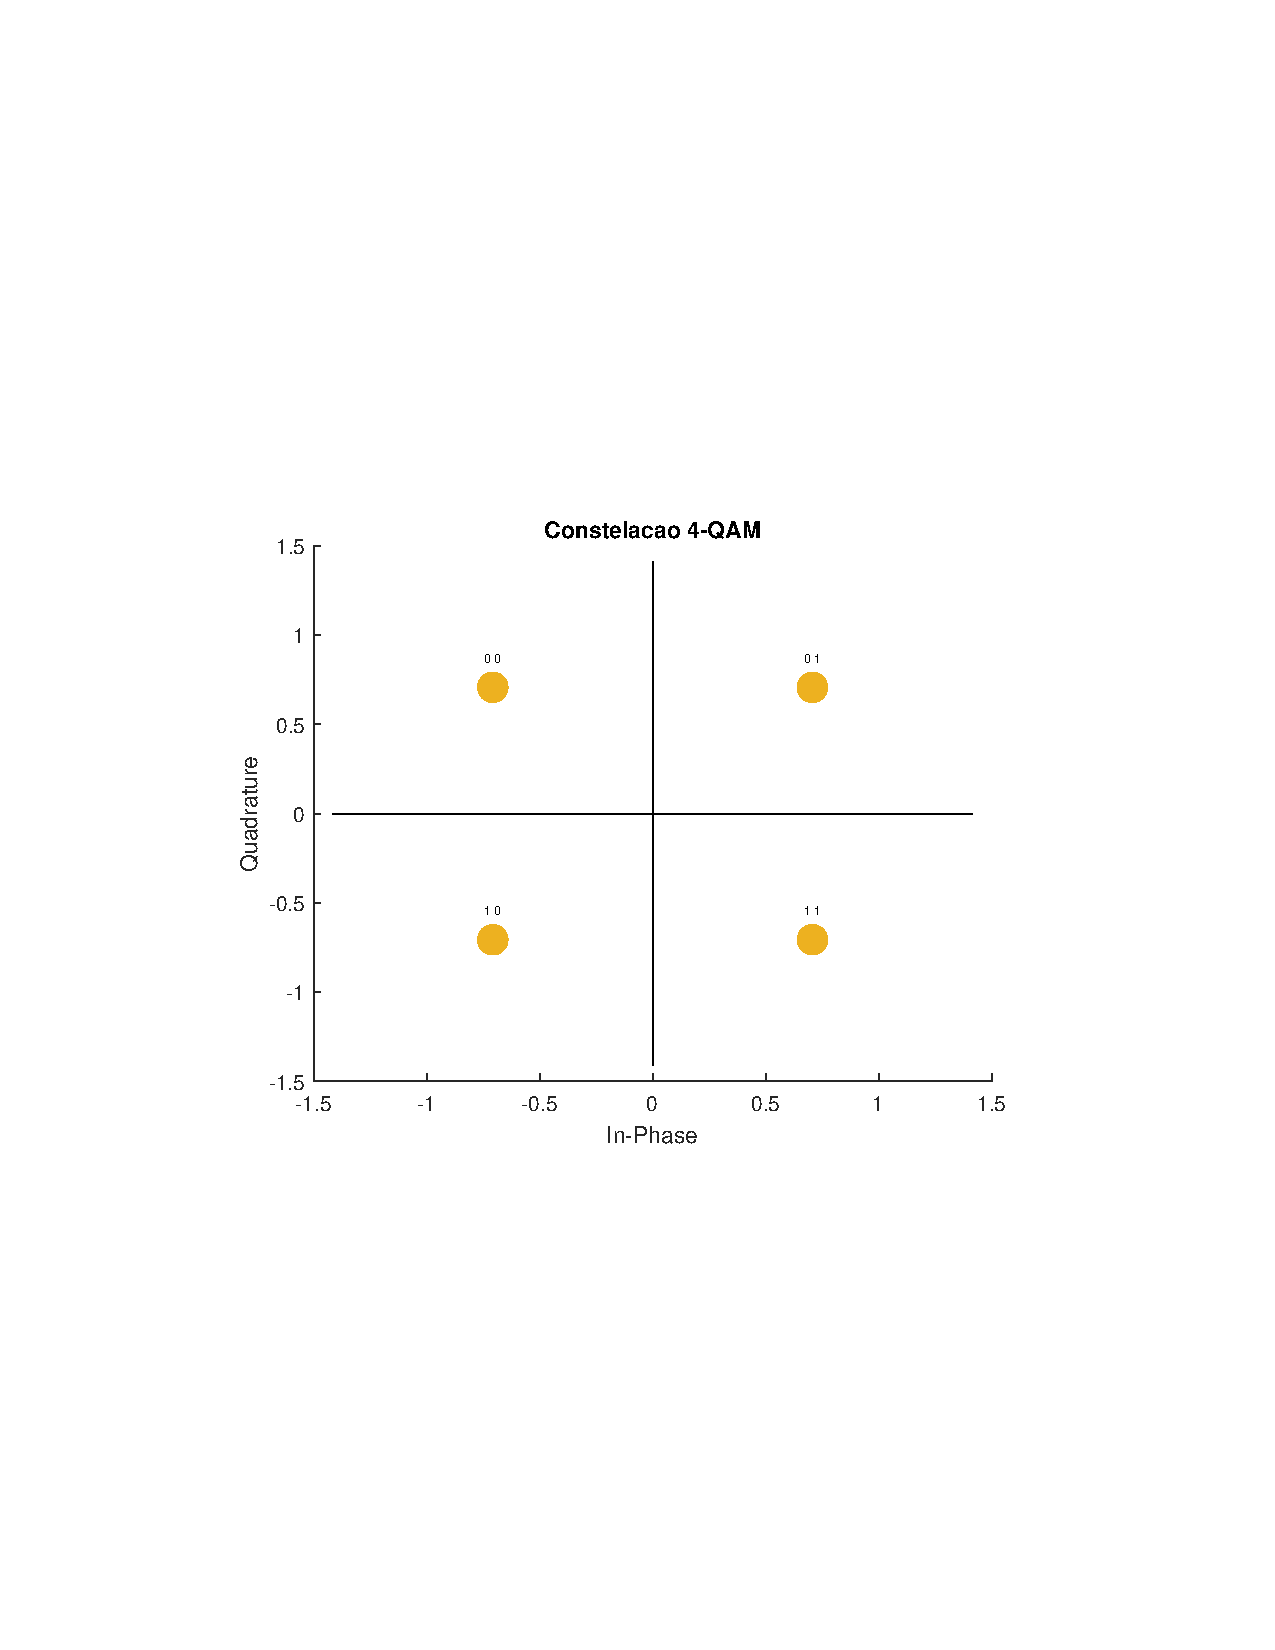
\includegraphics[width=1.0\textwidth,clip=true,trim={1.5cm 8.5cm 1.8cm 8.3cm}]{C:/Users/lukin/Documents/GitHub/Courses-HWs/Sistemas de Comunicacoes Digitais/matlab/problema1/fig/4_QAM_plot.pdf}
    \caption{Exemplo de 4-QAM plot.}
    \label{fig:4_QAM_plot}
\end{figure}

\begin{table}[!ht]
    \centering
    \begin{tabular}{|c|c|c|c|}
    \hline
    Decimal & Binário & Gray & Decimal \\ \hline
    0 & 00 & 00 & 0\\ \hline
    1 & 01 & 01 & 1\\ \hline
    2 & 10 & 11 & 3\\ \hline
    3 & 11 & 10 & 2\\ \hline
    \end{tabular}
    \caption{Tabela de tradução de binário para Gray com 2 bits.}
    \label{tab:Alfabeto_Gray}
\end{table}

Algoritmo para obter o código de Gray~\ref{alg:Gray}

% global change
\SetKwInput{KwData}{Entrada}
\SetKwInput{KwResult}{Saída}

\begin{algorithm}[!ht]
    \SetAlgoLined
    \KwData{Sequência de Bits $(b)$ - MSB}
    \KwResult{Sequencia em Código Gray $(g)$ - LSB}
    $n = 0$\;
    $K = \text{length}(b)$\;
    \While{$K > n$}{
        \eIf{$K==n$}{
            $g_{(K-n)} = b_{(K-n)}$ \;
            }{
            $g_{(K-n)} = b_{(K-n+1)} \otimes b_{(K-n)}$\;
        }
        $n=n+1$;\;
     }
     $g = flip(g)$\;
     \caption{Codificação de Gray}
     \label{alg:Gray}
\end{algorithm}

\clearpage



\begin{figure}[!ht]
    \centering
    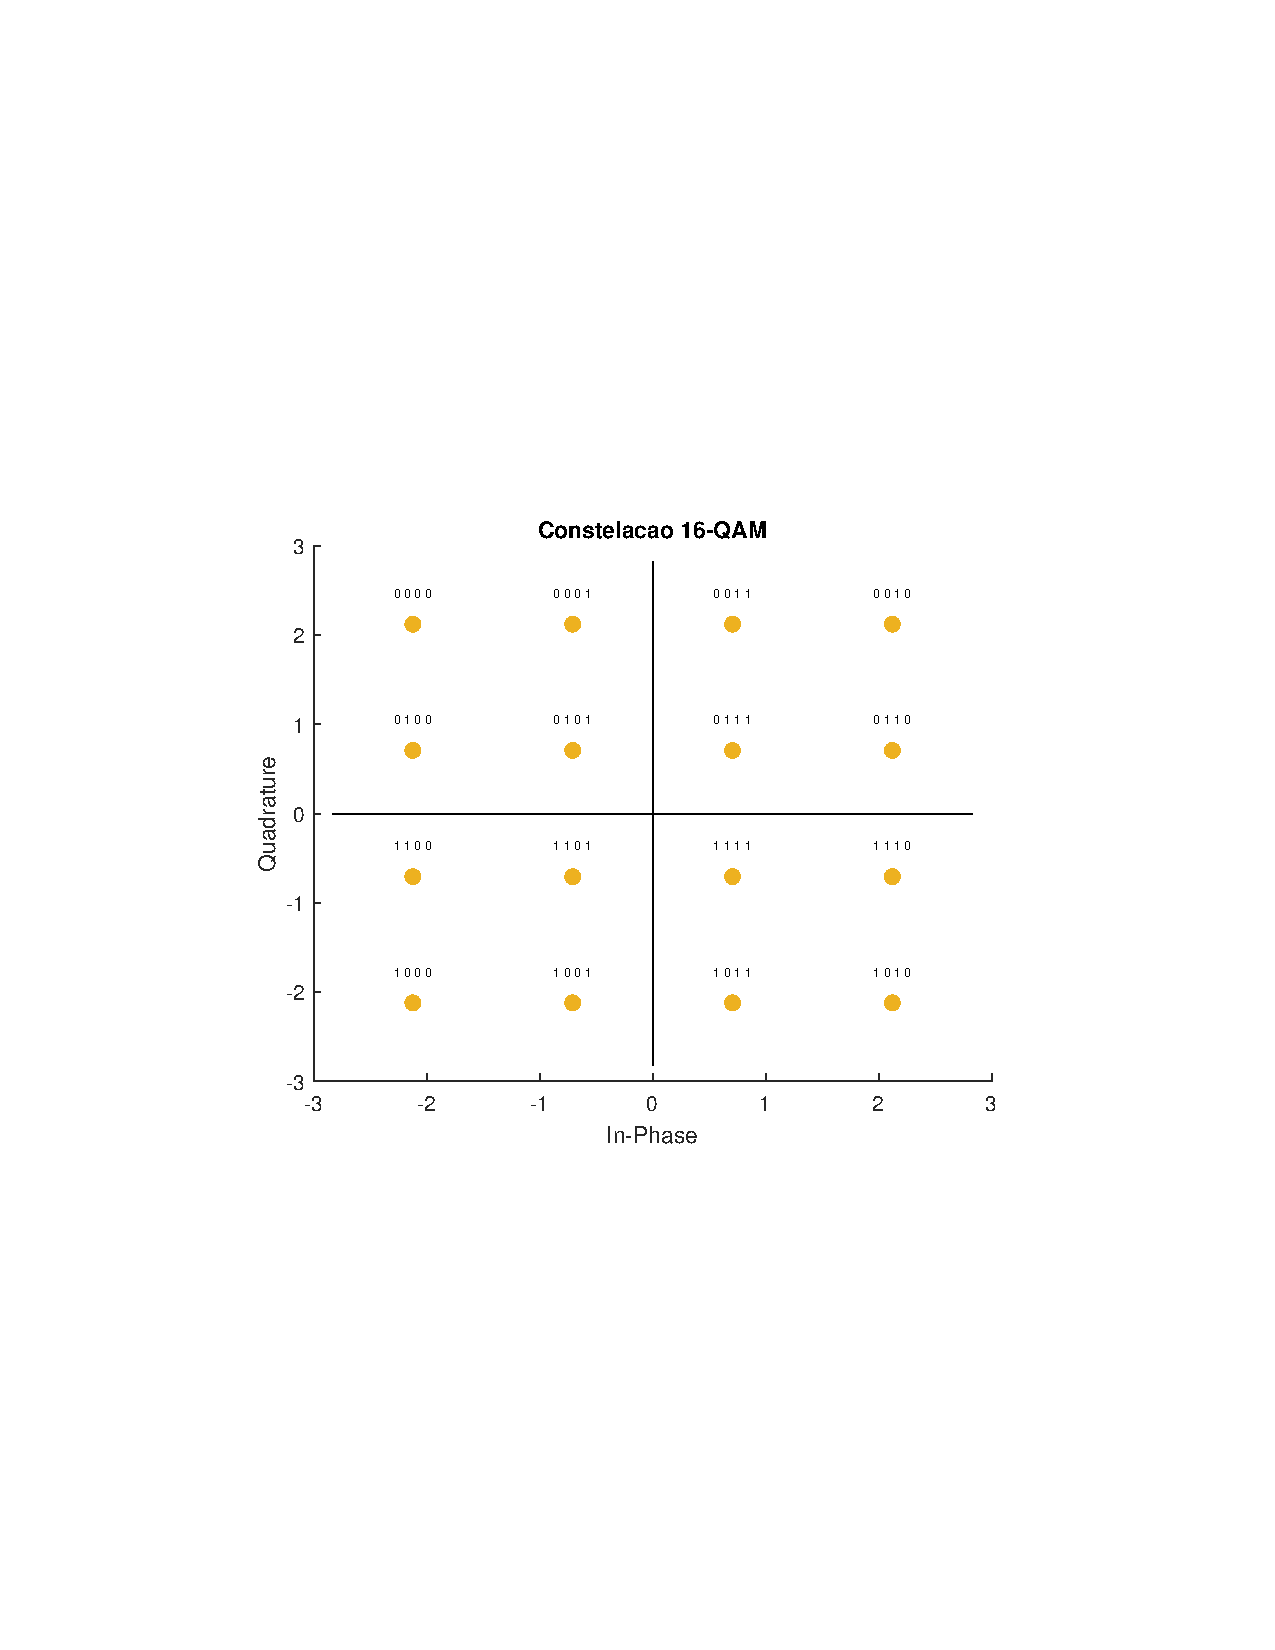
\includegraphics[width=1.0\textwidth,clip=true,trim={1.5cm 8.5cm 1.8cm 8.3cm}]{C:/Users/lukin/Documents/GitHub/Courses-HWs/Sistemas de Comunicacoes Digitais/matlab/problema1/fig/16_QAM_plot.pdf}
    \caption{Exemplo de 16-QAM plot.}
    \label{fig:16_QAM_plot}
\end{figure}

\begin{figure}[!ht]
    \centering
    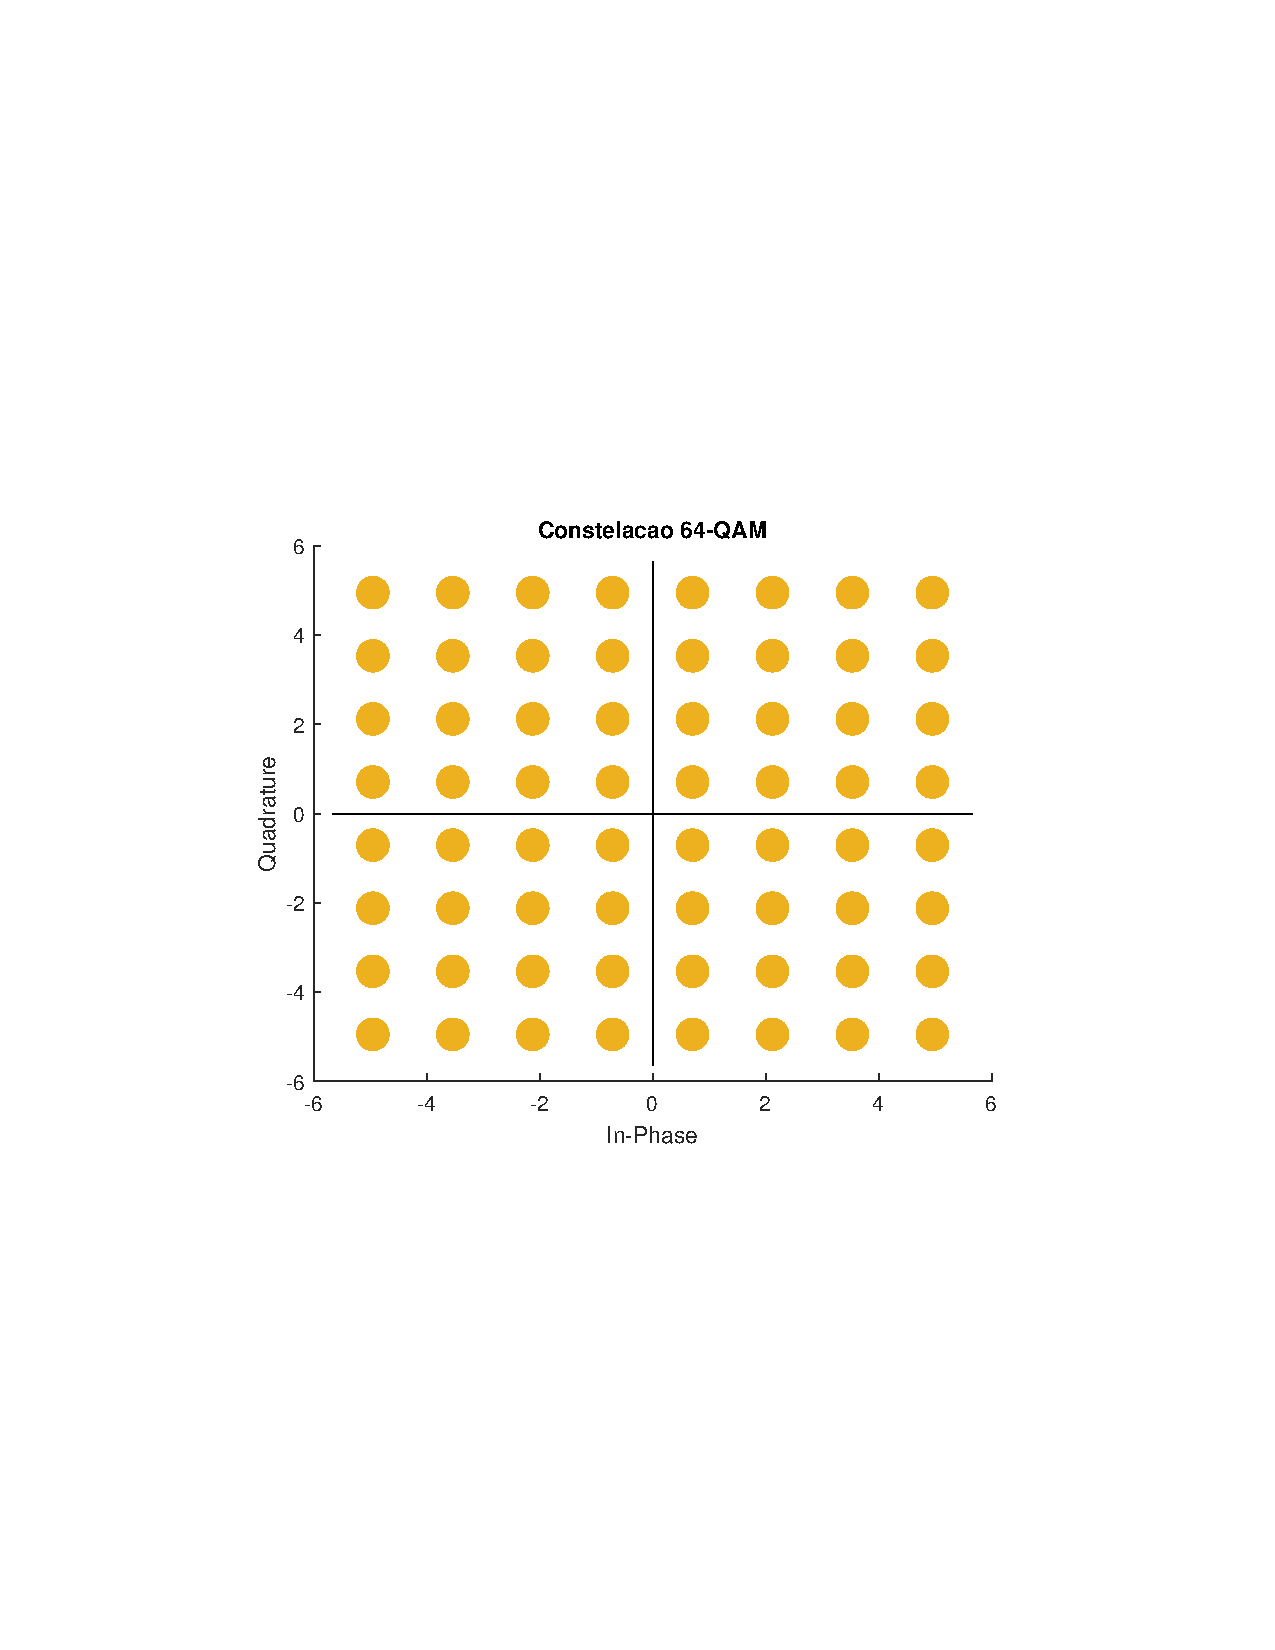
\includegraphics[width=1.0\textwidth,clip=true,trim={1.5cm 8.5cm 1.8cm 8.3cm}]{C:/Users/lukin/Documents/GitHub/Courses-HWs/Sistemas de Comunicacoes Digitais/matlab/problema1/fig/64_QAM_plot.pdf}
    \caption{Exemplo de 64-QAM plot.}
    \label{fig:64_QAM_plot}
\end{figure}

\clearpage

% -------------------------------------------------------------------
\subsubsection{Demodulador}

Considerando $\mathcal{E}_g = \int_{-\infty}^{\infty} |g(t)|^2 \,dt = 1$, a energia média da constelação pode ser calculada por $\epsilon$



%%
% Please add the following required packages to your document preamble:

\clearpage

Para calcular a probabilidade de erro $P(e)$ de cada constelação~\ref{eq:Pe_M_QAM} desenvolvida em~\cite{Cecilio}.
\begin{equation}
    P(e) = 4 \left(1-\frac{1}{\sqrt{M}}\right) Q\left(\sqrt{\frac{3}{M-1}\frac{E_s}{N_0}}\right) - 4\left(1-\frac{1}{\sqrt{M}}\right)^2 Q^2\left(\sqrt{\frac{3}{M-1}\frac{E_s}{N_0}}\right)
    \label{eq:Pe_M_QAM}
\end{equation}

Para valores mais elevados de \textit{SNR}, a equação da probabilidade do $M$-QAM pode ser reduzida para~\ref{eq:Pe_reduzida_M_QAM}, pois o segundo termo ao quadrado passa a ser irrelevante.
\begin{equation}
    P(e) = 4 \left(1-\frac{1}{\sqrt{M}}\right) Q\left(\sqrt{\frac{3}{M-1}\frac{E_s}{N_0}}\right)
    \label{eq:Pe_reduzida_M_QAM}
\end{equation}


\section{Conclusão e Resultados}

\clearpage

% Bibliografia
% LateX vai gerar as ``Referências'' automaticamente
% usando a função \cite{nome} do pacote BibTeX é possível
% "puxar todas as informações do arquivo 'refs.bib'
% O nome do arquivo é o primeiro parâmetro de cada referência
% Um exemplo esta é utilizado na primeira seção
% \AtNextBibliography{\small}             % To set a smaller font size for bibliography
\printbibliography[heading=bibintoc]    % Print the references

\end{document}